\documentclass[12pt, letterpaper]{article}
\usepackage[margin=0.9in]{geometry}

\usepackage{xcolor}

\usepackage{amsmath}
\usepackage{amssymb}
\usepackage{amsthm}
%\usepackage[utf8]{inputenc}
\usepackage[colorlinks]{hyperref}
\hypersetup {
  colorlinks=true,
  linkcolor=magenta
}
\usepackage{tocloft}
\usepackage{tikz-cd}

\usepackage[font=footnotesize ,skip=0pt]{caption}
\usepackage{graphicx}
\graphicspath{{figures/}}
\usepackage{float}


% amsthm setup
\theoremstyle{definition} % get rid of the ugly italics everywhere
\newtheorem{thm}{Theorem}[section] % number theorems by sections
\newtheorem{defn}[thm]{Definition} % use the same counter ``thm'' for all theorems.
\newtheorem{defnthm}[thm]{Definition-Theorem}
\newtheorem{cor}[thm]{Corollary}
\newtheorem{note}[thm]{Note}
\newtheorem{ex}[thm]{Example}
\newtheorem{notitle}[thm]{}
\newtheorem{choice}[thm]{Axiom of Choice}

% Useful math mode definitions
\def\img{\operatorname{img}}
\def\hom{\operatorname{Hom}}
\def\LABELMCK{}

\def\tr{\operatorname{tr}}
\newcommand{\mck}[1]{\ifdefined\LABELMCK(McKernan #1).\fi}
\def\gal{\operatorname{Gal}}
\def\GL{\operatorname{GL}}

% Put horizontal dots in the TOC
\renewcommand\cftsecleader{\cftdotfill{\cftdotsep}}
 

%title init.
\title{Physics 220 notes -- Group Theory for Physicists \\ (Mostly discrete groups)}
\author{David Moore}
\date{Updated \today}
 
\begin{document}

\maketitle

\tableofcontents

\section*{Introduction}

This is a set of notes written in conjunction with a UCSD Group Theory 
for Physicists course.
The actual course notes are 
\href{https://wucj.physics.ucsd.edu/teach/Phy220_2018/phy220.html}{available online here}.
The ``theorems'' in this document aren't necessarily theorems and the ``proofs'' just have to 
be convincing enough. 

There's also an emphasis on applications and examples. I try to write most of the actual theory in 
``definition-theorem-proof'' style, and the examples/applications in a more informal style.


\section{Groups}

\subsection{Basic Theory of Groups}
\begin{defn}
  A \emph{group} is a set $G$ together with a binary operation $\cdot:G\times G\to G$ such that:
  \begin{enumerate}
    \item $\forall_{a,b,c\in G}$, $(a\cdot b)\cdot c=a\cdot (b\cdot c)$.
    \item $\exists_{e\in G} \forall_{g\in G}$,  $e\cdot g=g$.
    \item $\forall_{g\in G} \exists_{g^{-1}\in G}: g\cdot g^{-1}=e$.
  \end{enumerate}
\end{defn}
\begin{thm} Basic theorems about groups:
  \begin{itemize}
    \item The identity element $e\in G$ is unique.
    \item Inverse elements are unique.
    \item $ge=g$
    \item $g^{-1} g=e$.
  \end{itemize}
\end{thm}
\begin{defn}
  Given a group $G$, a \emph{subgroup} $H\subseteq G$ is a subset of $G$ which itself is a group. 
  This is often written $H\leq G$.
\end{defn}
\begin{defn}
  Given a group $G$, subgroup $H\leq G$, and group element $g\in G$, a \emph{coset} is the set
  $gH=\{g h_1,g h_2,\ldots\}$. Note that $|g_1 H|=|H|$. (This is also called a 
    left-coset. You can also define right-cosets $Hg=\{h_1 g,\ldots\}$ but we don't 
  need them.)
\end{defn}
\begin{thm}
  $g_1 H$ and $g_2 H$ either share all their elements or none of their elements.
\end{thm}
\begin{proof}
  Suppose there is a common element $f\in g_1 H$ and $f\in g_2 H$. Then for some $h_1, h_2\in H$, $f=g_1 h_1=g_2 h_2$.
  Now let $g_2 h$ be any element of $g_2 H$. Using the formulas for $f$: 
  $g_2 h=f h_2^{-1} h=g_1\left( h_1 h_2^{-1} h\right)=g_1 h'$. So $g_2 H\subseteq g_1H$. The proof is symmetric, so in fact
  $g_1 H\subseteq g_2 H$ and the sets are equal.
\end{proof}
\begin{defn}
  Let $H\subseteq G$. The \emph{index} of the subgroup $H$ with respect to $G$, denoted $[H:G]$, is the number of cosets $gH$.
\end{defn}
\begin{thm}
  (Lagrange). For finite groups, if $H\leq G$, then $|G|/|H|$ is an integer and is equal to the number of cosets of $H$. 
  ie $|G|=[G:H]|H|$
\end{thm}
\begin{proof}
  Every element of $G$ belongs to some coset $gH$. These cosets cannot overlap (by the previous theorem), and the cosets are all
  of the same order. So we have partitioned the group $G$ into $n$ sets of size $|H|$, giving the relation $|G|=n|H|$. 
\end{proof}
\begin{defn}
  Given group $G $, a \emph{normal subgroup} $H\mathrel{\unlhd}G$ is a subgroup $H$ such that for every $g\in G$, $gH=Hg$.
\end{defn}
\begin{defnthm}
  Given a normal subgroup $H\mathrel{\unlhd}G$, the \emph{quotient group} is the set of cosets $G/H=\{gH | g\in G\}$ with the
  group operation $(g_1 H)\cdot(g_2 H)=(g_1\cdot g_2)H$. This is a well-defined group operation and is independent of which group elements
  you choose.
\end{defnthm}
\begin{defn}
  Given two groups $A,B$, a function $f:A\to B$ is called a \emph{group homomorphism} if
  $f(a_1\cdot a_2)=f(a_1)\cdot f(a_2)$. The \emph{kernel} of a group homomorphism is the 
  set of all elements of $A$ that map to the identity in $B$, $\ker f=\{a : f(a)=e\}$.
\end{defn}
\begin{defnthm}
  The kernel of a group homomorphism is a normal subgroup. 
\end{defnthm}
\begin{note}
  The easiest way to prove that a subgroup $N\mathrel{\unlhd}G$ is normal is to find a 
  homomorphism from $G$ to some other group with $N$ as its kernel.
\end{note}
\begin{defn}
  A \emph{simple group} is a group $G$ with no normal subgroups except for the trivial cases $\{e\}\mathrel{\unlhd} G$ and $G\mathrel{\unlhd}G$.
\end{defn}
\begin{defn}
  Given a group element $g\in G$, the \emph{conjugacy class} of $g$ is the set of all $xgx^{-1}$ where $x\in G$. That is: $C_g=\{x g x^{-1} : x\in G\}$.
\end{defn}


\subsection{Example: permutation groups}

\begin{defn}
  The symmetric group $S_n$ is the set of all permutations on $n$ elements. We have $|S_n|=n!$.
\end{defn}
\begin{defn}
  Every permutation is either even or odd, depending on whether you need an even or odd number of swaps to form the permutation. The group of all even permutations is known as
  the \emph{alternating group} $A_n$. It's a normal subgroup of $S_n$ of order $n!/2$.
\end{defn}
\begin{thm}
  $A_n$ is normal.
\end{thm}
\begin{proof}   Construct the map $f:S_n\to S_2$, which sends a permutation to the identity if it's even, and to the other element if it's odd. 
  Then $\ker f$ is precisely the alternating group $A_n$. Kernels of homomorphisms are
  normal subgroups, so $A_n$ is normal in $S_n$.
\end{proof}

\begin{note} (Cycle notation). A permutation that sends $1\mapsto 2$, $2\mapsto 3$ and $3\mapsto 1$ is a cycle of length 3, and 
  can be denoted by $(1\ 2\ 3)$. You can also compose cycles: $(1\ 2\ 3)(1\ 2)$ is the cycle which first swaps $1$ and $2$, 
  and then applies the three-cycle from before. We find $(1\ 2\ 3)(1\ 2)=(1\ 3)$. Every permutation can be written as the product of disjoint cycles,
  $(i_1\ i_2\ \cdots)(i_3\ i_4\ \cdots)\cdots\in S_n$.
\end{note}
\begin{note} (Two-row notation). The above permutation $(1\ 2\ 3)$ can be written as $\begin{pmatrix} 1 & 2 & 3 \\ 2 & 3 & 1\end{pmatrix}$. The numbers
  in the first row get send to the corresponding numbers in the second row. This notation makes it easier to multiply permutations by hand.
\end{note}
\begin{thm}
  If $g=(i_1\ i_2\ i_3\ \cdots)$ is a permutation written in cycle notation, then given a permutation $\tau$,  
  $\tau g \tau^{-1}=(\tau(i_1)\ \tau(i_2)\ \tau(i_3)\ \cdots)$. 
\end{thm}
\begin{proof}
  $\tau g \tau^{-1}$ is the permutation which sends $\tau(i_1)$ to $\tau( g(i_1))=\tau(i_2)$.
\end{proof}
\begin{cor}
  Conjugacy classes in $S_n$ are permutations with same cycle pattern.
\end{cor}
\begin{proof}
  The previous theorem shows that conjugation can't change the cycle pattern. Furthermore, for any two permutations with the same cycle structure, we can 
  find a third permutation to relate the two by conjugation. For example if $a=(1\ 2\ 3)(4\ 5)$ and $b=(5\ 4\ 3)(2\ 1)$, then the permutation 
  $\tau=\begin{pmatrix} 1 & 2 & 3 & 4 & 5 \\ 5 & 4 & 3 & 2 & 1 \end{pmatrix}$ has $\tau a \tau^{-1}=b$.
\end{proof}
\begin{cor}
  There are $p(n)$ conjugacy classes of $S_n$, where $p(n)$ is the number of unordered integer partitions of $n$.
  For example, $p(3)=3$ because $3$ can be written as $3$, $2+1$, or $1+1+1$. 
\end{cor}
\begin{proof}
  Each partition corresponds one-to-one to a particular cycle structure, 
  which corresponds one-to-one to a conjugacy class. 
\end{proof}
\begin{note}
  There isn't a general formula for $p(n)$, but there's
  an asymptotic formula given by Hardy and Ramanujan:
\begin{equation*}
  p(n)\sim \frac{1}{4 n \sqrt{3}} \exp \left(\pi \sqrt{\frac{2n}{3}}\right)
\end{equation*}
\end{note}

\begin{defn}
  A Young diagram is a diagram in one-to-one correspondence with an unordered partition of $N$. It consists of $N$ squares
  in rows such that there are $n_1$ squares in the first row, $n_2\leq n_1$ squares in the second row, and so on. This is a trivial 
  definition, but it will be indispensible for thinking about combinatorics later on.

  \begin{figure}[H]
\centering
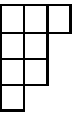
\includegraphics[width=0.1\textwidth]{fig1-young}
\caption*{A Young diagram corresponding to the partition $8=3+2+2+1$}
\label{figure-2}
\end{figure}

\end{defn}
\begin{thm} (Conjugacy classes using Young tableaux).
  Let $c$ be a conjugacy class of $S_N$. Suppose the cycle structure of $c$ will have $n_1$ cycles of length 1, $n_2$ cycles of length 2, and so on.
  Then $$|c|=\frac{N!}{\prod_j (j)^{n_j} (n_j!)}$$
\end{thm}
\begin{proof}
  Think about filling in the boxes of the corresponding Young diagram. There are $N!$ ways to fill in the $N$ boxes with the numbers one through $N$,
  but some correspond to the same permutations. If there are $n_j$ cycles of length $j$, then we have counted each of these $n_j!$ times (we can swap any two rows of the same length without changing the permutation). Furthermore,
  for every cycle of length $j$ like $(1\ 2\ \cdots\ j)$, we've included labelings like $(j\ 1\ 2\ \cdots)$, $(2\ \cdots\ j\ 1)$, and so on. There are
  $j$ of these equivalent labelings, so for each cycle of length $j$ we have overcounted by another factor of $j$. This means that overall, we have overcounted
  by a factor of $\prod_j j^{n_j} (n_j!)$. 
\end{proof}

  \begin{figure}[H]
\centering
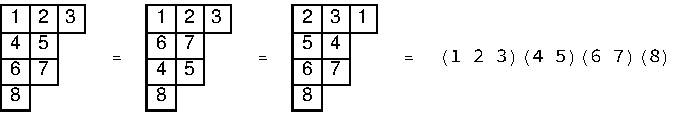
\includegraphics[width=0.7\textwidth]{fig2-youngequivalent}
\caption*{Several ways of labeling the Young diagram to get the same permutation}
\label{figure-1}
\end{figure}


\section{Representations}
We'll only consider vector spaces over $\mathbb{R}$ or $\mathbb{C}$.
\subsection{Theory and the Schur theorems}

\begin{defn}
  Let $V$ be a vector space. Then $\GL(V)$, the \emph{general linear group} on $V$ is the group of all invertible linear operators on $V$.
\end{defn}
\begin{defn}
  Given a group $G$ and vector space $V$, a \emph{representation} is some group homomorphism $M:G\to \GL(V)$. 
  The representation is often denoted $M(G)$.
\end{defn}

\begin{defn}
  \label{intertwining}
  Let $G$ be a group, and let $M:G\to \GL(V_1)$ and $N:G\to \GL(V_2)$ be two
  representations of $G$. A linear map $L:V_1\to V_2$ is called an \emph{intertwining map}
  if, for all $g\in G$, $L(M(g))v_1=N(g) L(v_1)$. 

  In matrix notation, if $M(g)$ has dimensions $m\times m$ and $N(g)$ has dimensions $n\times n$, 
  then $L$ is an $n\times m$ matrix such that $L M(g)=N(g)L$.

  Intertwining maps provide the way to relate representations on different vector spaces.
\end{defn}

\begin{defn}
  \label{equivalent}
  Let $G$ be a group, and let $M:G\to \GL(V_1)$ and $N:G\to \GL(V_2)$ be two
  representations of $G$. The representations $M$ and $N$ are said to be \emph{equivalent}
  if there exists an invertible intertwining map $L:V_1\to V_2$. We also say that the two representations
  are \emph{isomorphic}.
\end{defn}

\begin{thm}
  If $V_1=V_2=V$, then two representations are equivalent if and only if for some 
  matrix $L$ and all $g\in G$, $N(g)=L M(g)L^{-1}$. 
\end{thm}
\begin{proof}
  Using the same notation as in the last two definitions, $L$ is an 
  invertible linear map. We have $L M(g)=N(g) L$, or $L M(g)L^{-1}=N(g)$. 
  So the whole business with intertwining maps is just a fancy way of saying the matrices are
  conjugate to each other.
\end{proof}

\begin{defn}
  Given a representation $M:G\to \GL(V)$, a vector subspace $U\subseteq V$ is called an invariant subspace if
  $M(g)U=U$ for all $g\in G$. Representations always have the trivial invariant subspaces $\{\vec{0}\}$ and $V$.
\end{defn}

\begin{defn}
  A representation $M:G\to \GL(V)$ is called \emph{reducible} if it has a nontrivial invariant subspace. 
  That is, if it has an invariant which is neither $\{\vec{0}\}$ or $V$.
  
  A representation that is not reducible is called \emph{irreducible}. The word ``irrep'' is short for irreducible representation.
\end{defn}

\begin{defn}
  Take a group $G$, representation $R_1$ over vector space $V_1$, and representation $R_2$ over vector space $V_2$,
  the \emph{direct sum representation} $R=R_1\oplus R_2$ is the representation of $G$ over vector space
  $V_1\oplus V_2$, with action $R(g)(v_1,v_2)=(R_1(g)v_1,R_2(g)v_2)$. 
\end{defn}

\begin{defn}
  Take a group $G$, representation $R_1$ over vector space $V_1$, and representation $R_2$ over vector space $V_2$,
  the \emph{tensor product representation} $R=R_1\otimes R_2$ is the representation of $G$ over vector space
  $V_1\otimes V_2$, with action $R(g)(v_1\otimes v_2)=(R_1(g)v_1)\otimes(R_2(g)v_2)$. (To prove  this is well defined,
  use the universal property of the tensor product).
\end{defn}
\begin{note}
  We can also define the direct sum of two representations of two different groups. In that case we wind up with 
  a representation of $G_1\times G_2$. This is not used too often in physics; usually we just care about different representations
  of the same group $G$.
\end{note}
\begin{defn}
  A representation which is a direct sum of irreps is called \emph{completely reducible}.
\end{defn}

\begin{ex} (A reducible representation which is not completely reducible). The group of real numbers under addition has a representation by the
  two-by-two matrices $\begin{bmatrix} 1 & a \\ 0 & 1\end{bmatrix}$. The vector subspace spanned by $(1,0)$ is fixed under the action of these matrices,
  so this representation is reducible. However, there is no other invariant subspace and therefore this representation cannot be a direct sum of invariant subspaces.

  We don't need to worry much about cases like this though. We will prove that any representation of a finite group is equivalent to a unitary 
  representation, and that any reducible unitary representation is also completely
  reducible.
\end{ex}



\begin{thm}
  Schur's lemmas:
  \begin{enumerate}
    \item Let $M_1:G\to V_1$ and $M_2:G\to V_2$ be two irreps. Let $\phi$ be an intertwining map.
      Then either $\phi=0$ or $\phi$ is an isomorphism.
    \item Let $M:G\to V$ be an irrep, and let $\phi:V\to V$ be an intertwining map from $V$ to itself.
      Then $\phi=\lambda I$ for some $\lambda\in\mathbb{C}$.
  \end{enumerate}
\end{thm}

\begin{proof}
  {\bf Part 1}. Note that the kernel of $\phi$ is an invariant subspace of $M_1$, and the image of $\phi$  is an invariant
  subspace of $M_2$. So we either have $\ker \phi=V_1$ and $\img \phi=0$ (so $\phi=0$), or $\ker \phi=0$ and $\img \phi=V_2$
  (so $\phi$ is an isomorphism). \qed

  {\bf Part 2}. $\phi$ must have some eigenvalue $\lambda$ for which $\det (\phi-\lambda I)=0$. But then the map 
  $\phi-\lambda I$ has a nonempty kernel, so that its kernel must be the entirety of $V_1$. Then $\phi-\lambda I=0$. 
\end{proof}

\begin{cor}
  Schur's lemmas in matrix notation:
  \begin{enumerate}
    \item Let $M_1(g)$ be an $m_1\times m_1$ irrep, and let $M_2$ be an $m_2\times m_2$ dimensional irrep. Let $L$ be an
      $m_1\times m_2$ matrix such that for all $g$, $M_1L=LM_2$. Then either $L=0$ or $M_1$ and $M_2$ are equivalent representations.
    \item Let $M$ be an irrep, and let $L$ be a matrix that commutes with all $M(g)$. Then $L$ is proportional to the identity matrix.
  \end{enumerate}
\end{cor}

\begin{defn} (Unitary representation)
  Let $M$ be a representation on a vector space $H$ with inner product $\langle cv_1,v_2\rangle=c^*\langle v_1,v_2\rangle$. The
  adjoint operator $M^\dagger$ is the operator for which $\langle M^\dagger v_1,v_2\rangle=\langle v_1,Mv_2\rangle$ for all $v_1,v_2\in H$. 
  If each $M^\dagger=M^{-1}$, then $M$ is called a \emph{unitary representation}.
\end{defn}

\begin{thm}
  \label{unitaryrep}
  Any linear representation of a finite group is equivalent to a unitary transformation.
\end{thm}
\begin{proof}
  Let $H$ be a Hilbert space with inner product $\langle v_1,v_2\rangle_1$. Let $M(g)$ be a representation on a finite group. 
  Define a new inner product $\langle v_1,v_2\rangle_2=\sum_g\langle M(g)v_1,M(g)v_2\rangle_1$. The representation $M(g)$ is 
  unitary with respect to this inner product, because: 
  
  \begin{align*}
    \langle v_1,M(h)v_2\rangle_2&=\sum_g\langle M(g)v_1,M(gh)v_2\rangle_1\\
    &=\sum_{g'}\langle M(g' h^{-1})v_1,M(g')v_2\rangle_1\\
  &=\sum_{g}\langle M(g)M(h^{-1})v_1,M(g)v_2\rangle_1\\
  &=\langle M(h)^{-1}v_1,v_2\rangle_2
  \end{align*}
\end{proof}

\begin{note}
  It's surprisingly tedious to link the abstract definition/theorem to actual matrices. An
  alternate proof of theorem \ref{unitaryrep} would involve finding a matrix $X$ such
  that $X M(g) X^{-1}$ is a unitary matrix.

  In this case the intertwining map was trivial, since all we did was reinterpret our Hilbert space as a space with a different inner product.
  If we to write this in terms of matrices then we have to implement a change of basis, and there's a small mountain of notation.

  We can use theorems from linear algebra to find our orthonormal bases: $\langle e_i,e_j\rangle_1=\delta_{ij}$, 
  and $\langle \hat{e}_i,\hat{e}_j\rangle_2=\delta_{ij}$. Then:
  
  \begin{enumerate}
    \item $v=\langle e_i,v\rangle_1 e_i$ and $v=\langle \hat{e}_i,v\rangle_2 \hat{e}_i$ \emph{(The orthonormal bases are complete)}
    \item $M_{ij}^g=\langle e_i,M(g) e_j\rangle_1$ and $\hat{M}^g_{ij}=\langle \hat{e}_i,M(g)\hat{e}_j\rangle_2$ \emph{(Matrix definitions)}
    \item $M(g) e_j=e_i M_{ij}^g$ \emph{(Consequence of completeness)}
    \item $X_{ij}=\langle e_i,\hat{e}_j\rangle_1$ (Definition of the change of basis matrix)
    \item $(X^{-1})_{ij}=\langle \hat{e}_i,e_j\rangle_1$ \emph{(Change of basis matrix inverse. As a proof consider $e_i=e_k\langle e_k,\hat{e}_j\rangle_1\langle \hat{e}_j,e_i\rangle_1$)}
    \item $\hat{e}_j=e_i X_{ij}$ and $e_j=\hat{e}_i (X^{-1})_{ij}$ \emph{(consequence of completeness)}
    \item $\langle e_i,e_j\rangle_2=(X^{-1})_{ki}^* (X^{-1})_{kj}=((X^{-1})^\dagger X^{-1})_{ij}$
  \end{enumerate}

  Then, in totally exhaustive detail:

  \begin{align*}
    \hat{M}_{ai}(h)&=\langle \hat{e}_a, M(h)\hat{e}_i\rangle_2\\
    &=\sum_g\langle M(g)\hat{e}_a,M(gh)\hat{e}_i\rangle_1\\
    &=\sum_g\langle M(g)e_b X_{ba},M(gh)e_j X_{ji}\rangle_1\\
    &=\sum_g\langle M(g)e_b X_{ba},M(g)e_kM^h_{kj} X_{ji}\rangle_1\\
    &=X_{ba}^*M^h_{kj}X_{ji}\sum_g\langle M(g)e_b,M(g)e_k\rangle_1\\
    &=X_{ba}^*M^h_{kj}X_{ji}\langle e_b,e_k\rangle_2 \\
    &=X_{ba}^*M^h_{kj}X_{ji}((X^{-1})^\dagger X^{-1})_{bk} \\
    &=X_{ba}^*((X^{-1})^\dagger X^{-1})_{bk}M^h_{kj}X_{ji} \\
    &=(X^\dagger)_{ab}((X^{-1})^\dagger X^{-1})_{bk}M^h_{kj}X_{ji} \\
    &=(X^{-1}M^hX)_{ai}
  \end{align*}
\end{note}
\begin{cor}
  If $M^g_{ij}$ is a matrix representation of a finite group, there exists a matrix $X$ such that $X_{ij} M^g_{jk} X^{-1}_{k\ell}$ is a unitary matrix representation 
  of $G$.
\end{cor}


\begin{thm} \emph{(Irrep orthogonality relation)}
  Let $M$ and $N$ be two irreducible unitary matrix representations of a group $G$. Then the following two relations hold:
  
  \begin{enumerate}
    \item if $M$ and $N$ are inequivalent representations, $\sum_{g\in G} M^*_{\mu \rho}(g) N_{\nu \lambda}(g)=0$.
    \item $\sum_{g\in G} M^*_{\mu \rho}(g) M_{\nu \lambda}(g)=\frac{|G|}{m} \delta_{\mu\nu}\delta_{\rho\lambda}$, where $m$ is the dimension of the representation.
  \end{enumerate}
\end{thm}
\begin{proof}
  Define the matrices ${Y}(\mu \nu)$ to have components ${Y}(\mu \nu)_{\rho \lambda}=\delta_{\mu\rho}\delta_{\nu \lambda}$.
  Then define the matrices ${X}(\mu\nu)=\sum_{g\in G} M(g^{-1}) Y(\mu\nu) N(g)$. First, note that 
  $X(\mu\nu)_{\rho\lambda}=\sum_{g\in G} M_{\mu\rho}(g)^* N_{\nu\lambda}(g)$ (expand into indices and apply the fact that $M$ is a unitary matrix). 
  Next, note:

  \begin{align*}
    M(h)X(\mu\nu)&=\sum_g M(h g^{-1}) Y(\mu\nu)N(g)\\
    &= \sum_{g'} M(g'^{-1})Y(\mu\nu) N(g' h)\\
    &= X(\mu\nu)N(h)
  \end{align*}

  where the substitution $g'^{-1}=h g^{-1}$ was made.

  In the case that $M$ and $N$ are inequivalent representations, Schur's lemma gives $X(\mu\nu)=0$ so that $\sum_{g\in G} M_{\mu\rho}(g)^* N_{\nu\lambda}(g)=0$ and the theorem is proved.

  In the case that $M=N$, we have shown that $X(\mu\nu)$ commutes with all elements $M(h)$, and Schur's other lemma gives that each $X$ must be proportional to the identity matrix: $X(\mu\nu)=c(\mu\nu) I$.
  We can take the trace of $X(\mu\nu)$ to get the constant: 
  
  \begin{align*}
    m c(\mu\nu)&=\tr(X(\mu \nu))\\
    &=\sum_g \tr(M(g^{-1}) Y(\mu\nu) M(g))\\
    &=\sum_g \tr(Y(\mu\nu))\\
    &=|G|\delta_{\mu \nu}\\
  \end{align*}

  So we have shown $X(\mu \nu)=\frac{|G|}{m}\delta_{\mu\nu} I$, and therefore 
  \begin{equation*}
    \sum_{g\in G} M_{\mu\rho}(g)^* N_{\nu\lambda}(g)=X(\mu\nu)_{\rho\lambda}=\frac{|G|}{m}\delta_{\mu \nu}\delta_{\rho\lambda}
  \end{equation*}
\end{proof}

\begin{note}
  Conspicuously missing is the case $N(g)=Q M(g)Q^{-1}$ for all $g$.  If you plug this into the orthogonality relation, you get 
  $\sum_{g\in G} M^*_{\mu \rho}(g) (Q M(g) Q^{-1})_{\nu \lambda}=\frac{|G|}{m} Q_{\nu\mu}(Q^{-1})_{\rho\lambda}$. So you can't apply this relation to 
  two equivalent irreps. However, if you add the caveat that $M$ and $N$ are either inequivalent or exactly equal, we can write 
  The Great Orthogonality Relation in one line:

  \begin{equation}
    \sum_{g\in G} M^*_{\mu \rho}(g) N_{\nu \lambda}(g)=\frac{|G|}{m} \delta_{MN}\delta_{\mu \nu}\delta_{\rho \lambda}
    \label{orthogonality}
  \end{equation}
\end{note}



\section{Characters}

\subsection{Basic Theorems and Theory}

We'll consider unitary matrix representations unless otherwise stated.

\begin{defn}
  Let $f:G\to \mathbb{C}$ be some function. If $f(g)=f(h^{-1} g h)$ for all $h,g\in G$, then $f$ is called a \emph{class function}.
  The space of all class functions is an $n_c$-dimensional vector space, where $n_c$ is the number of conjugacy classes of $G$. 
\end{defn}
\begin{defn}
  For a matrix representation $M(g)$, define the \emph{character} $\chi_M(g)=\tr M(g)$. $\chi_M$ is a class function, because 
  $\tr M(h g h^{-1})=\tr M(h)M(g)M(h^{-1})=\tr M(g)$.
\end{defn}
\begin{thm} (Orthogonality of characters). 
  \begin{equation*}
    \sum_{g\in G} \chi_M(g)^* \chi_N(g)=|G|\delta_{MN}
  \end{equation*}
   \label{orthogonality2}
\end{thm}
\begin{proof}
  \begin{align*}
    \sum_{g\in G} \chi_M(g)^* \chi_N(g)&= \sum_g M^*_{\rho\rho}(g) N_{\mu\mu}(g)\\
    &= \frac{|G|}{m}\delta_{MN} \delta_{\rho\mu}\delta_{\rho\mu}\\
    &= \frac{|G|}{m}\delta_{MN} \delta_{\rho\rho}\\
    &= |G|\delta_{MN}
  \end{align*}
\end{proof}
\begin{cor}
  Two irreps are equivalent if and only if they have the same characters.
\end{cor}
\begin{proof}
  If two irreps are equivalent, the cyclicity of the trace immediately means they have the same characters. ($\tr N^{-1} M N = \tr M N N^{-1}$)

  If they have the same characters, then $\sum_g \chi_M(g)^* \chi_{M'}(g)>0$, so that they can't be inequivalent.
\end{proof}
\begin{cor}
  Suppose $D(g)$ is a reducible representation, and let $M$ label the irreducible representations of $G$. 
  We may write write $X^{-1}D(g)X=\oplus a_M M(g)$, $a_M$ being the number of times the irrep $M$ appears in $D$.
  Then $\chi_D(g)=\sum_M a_M \chi_M(g)$, and orthogonality gives $a_M=\frac{1}{|G|} \sum_g \chi_M^*(g) \chi_D(g)$. That is, we can figure out what a reducible representation 
  is built out of by taking inner products of the characters.
  \label{innerrep}
\end{cor}
\begin{cor}
  A representation of a finite group is irreducible if and only if $\sum_g |\chi_M(g)|^2=|G|$. 
\end{cor}
\begin{proof}
  If we have an irrep, then the orthogonality theorem \ref{orthogonality2} shows the 
  formula holds.

  Now suppose $\sum_g |\chi_M(g)|^2\neq |G|$. Using the previous corollary we can take
  inner products with all the irreps, and we must find that two or more irreps
  appear in the direct sum, so that $M$ is reducible.
\end{proof}
\begin{thm}
  Let $j$ run over all unitary irreps of a finite group $G$, where each nonequivalent irrep has dimension $m_j$. 
  Then $\sum m_j^2=|G|$.
\end{thm}
\begin{proof}
  Let's construct a $|G|$-dimensional representation of $G$ called the regular representation $M^R$. 
  Our $|G|$-dimensional vector space is called ``group space''. We let every element of $G$ correspond to
  another orthonormal basis vector, so we can write vectors as $\sum_g c_g g$.
  
  Let $f,g,h\in G$, and note that we can
  use these as indices as well as arguments.
  Define $M^R_{f, g}(h)=1$ if $g=fh$ and zero otherwise. ie, $M^R_{f, g}(h)=\delta_{g,fh}$. This forms a representation, because\dots
  \begin{align*}
    M^R_{f, g}(h) M^R_{g, i}(k)&= \delta_{g,fh}\delta_{i,gk}\\
    &=\delta_{i,fhk}\\
    &= M^R_{f,i}(hk)
  \end{align*}
  
  The only way to get a nonzero trace for this is if $f=fh$ for some $h,f$, in which case $h$ is the identity and
  the trace is $|G|$.

  Now decompose $M^R$ into irreps as above. We have $a_j=\frac{1}{|G|}\sum_g \chi_j^*(g) \chi_c(g)=\frac{1}{|G|} \chi_j^*(e)\chi_c(e)=m_j$,
  where $m_j$ is the dimension of the $j$th irrep.

  So, from corollary \ref{innerrep}, $|G|=\chi_c(e)=\sum_j a_j \chi_j(e)=\sum_j m_j^2$.
\end{proof}
\begin{thm}
  Characters form a complete basis of class function space.
\end{thm}
\begin{proof}
  Let $F(g)$ be any class function, ans suppose $F(g)$ is a class function orthogonal to every
  character $\chi_M$ for irreps $M$. We will show $F(g)=0$ identically. 

  Define $\phi_M=\sum_g F(g)^* M(g)$. Note:
  $$M(h)\phi_M M(h)^{-1}=\sum_g F(g)^* M(hgh^{-1})=\sum_g F(h^{-1}gh)^* M(g)=\phi_M$$
  If $M$ is an irrep, Schur's lemma gives $\phi_M=\lambda I$, and if we take traces we find $m\lambda=\sum_g F(g)^* \chi_M(g)$,
  which is zero by assumption. So for every irrep, $\phi_M=0$.
  
  Now consider the regular representation on group space again. Consider $\phi_M^R$ acting on the basis vector corresponding to the identity element $e$.
  $M^R(g) e=g$, so $\phi_M^R e=\sum_g F(g)^* g$. But $M^R$ is conjugate to a direct sum of irreps, so we can write 
  $X^{-1}\phi_M^R X=\sum_g F(g)^* \bigoplus_M M(g)=\bigoplus_M \phi_M$ where each irrep occurs multiple times in the direct sum. But each term in the sum is equal to zero!
  So $0=\sum_g F(g)^* g$, and by linear independence $F(g)=0$ for all $g$.
\end{proof}

\begin{cor} (Completeness relation):
  $$\frac{|G|}{|C_\beta|}\delta_{\alpha,\beta}=\sum_j  \chi_j(C_\alpha) \chi_j(C_\beta)^*$$
  Where $C_\alpha$ are the conjugacy classes of $G$, the label $\alpha$ runs over conjugacy classes, and the label $j$ runs over all irreps.
  \label{completeness}
\end{cor}
\begin{proof}
  Since the characters form a complete basis of class function space, we can write $F(g)=\sum_j a_j \chi_j(g)$ for some coefficients $a_j$. 
  Choose $F(C_\alpha)=\delta_{\alpha,\beta}$, that is $F(g)$ is one if $g\in C_\beta$ and zero otherwise. 

  Multiply both sides by $\chi_k(g)^*$ and sum over $g$ to figure out $a_j$. 
  On the righthand side we can use the orthogonality relation \ref{orthogonality2}:
  $\sum_g \sum_j \chi_k^*(g) a_j \chi_j(g)=\sum_j |G| a_j \delta_{kj}=|G|a_k$. Now work on the left-hand side:

  \begin{align*}
    \sum_g \chi_k(g)^* F(g) &=\sum_\alpha |C_\alpha| \chi_k(C_\alpha)^* F(C_\alpha)\\
    &=\sum_\alpha |C_\alpha| \chi_k(C_\alpha)^* \delta_{\alpha \beta}\\
    &=|C_\beta| \chi_k(C_\beta)^*
  \end{align*}

  Setting the two sides equal, we find $a_j=\frac{|C_\beta|}{|G|} \chi_k(C_\beta)^*$, and so:
  $$\frac{|G|}{|C_\beta|}\delta_{\alpha,\beta}=\sum_j  \chi_j(C_\alpha) \chi_j(C_\beta)^*$$
\end{proof}

\begin{defn} (Self-conjugate representations).
  If $M(g)$ is an irrep, then $M(g)^*$ is also an irrep. If $M(g)^*$ is similar to $M(g)$, then $M$ is called a \emph{self-conjugate} 
  representation. Otherwise $M$ is called a \emph{complex representation}.

  If $M(g)$ is self-conjugate and there is a basis where all of its entries are real, then $M(g)$ is called a \emph{real representation}.
  If no such basis exists, $M(g)$ is called a \emph{pseudo-real representation}. (because $X^{-1} M(g)^* X=M(g)$ looks a bit like the 
  equation $c^*=c$)
\end{defn}

\begin{thm}
  If $M(g)$ is a self-conjugate irrep, and $X^{-1} M(g)^* X=M(g)$, then $X$ is symmetric if $M$ is a real representation and antisymmetric if $M$ 
  is a pseudoreal representation.
\end{thm}
\begin{thm}
  \begin{equation*}
    \frac{1}{|G|}\sum_g \chi(g^2)=
\begin{cases} 
  1 & M\text{ is real} \\
  -1 & M\text{ is pseudoreal} \\
  0 & M\text{ is complex} \\
   \end{cases}
  \end{equation*}
\end{thm}
\begin{defn}
  A conjugacy class $C_g$ is called self-conjugate
  if for all $h\in C_g$, $h^{-1}\in C_g$.
\end{defn}
\begin{thm}
  The number of self-conjugate classes is equal to the number of self-conjugate irreps.
\end{thm}

\begin{defn} (Character table)
  A Character table is a square table. Each column represents a different conjugacy class, and each row is a different irrep. 
  Its entries are $\chi_M(C_\alpha)$. For example:

\begin{equation*}
 \begin{array}{c || c c c} 
   & \{e\} & C_1 & C_2 \\ 
 \hline
 M_1 & \chi_1(e) & \chi_1(C_1) & \chi_1(C_2) \\ 
 M_2 & \chi_2(e) & \chi_2(C_1) & \chi_2(C_2) \\
 M_3 & \chi_3(e) & \chi_3(C_1) & \chi_3(C_2)  
\end{array}
\end{equation*}

There are lots of rules we've derived, summarized here. 
Let $j$ be an index that goes over irreps, $m_j$ be the dimension of the jth irrep,
  $n_c$ be the number of conjugacy classes of $G$. Let $\alpha$ be an index that goes over conjugacy classes and let $C_\alpha$ be the 
  $\alpha$th conjugacy class.
  \begin{enumerate}
    \item $\chi_j(e)=m_j$ (The first column of the character table gives the dimension of each irrep)
    \item $|G|=\sum_j m_j^2$ (the sum of squares of each dimension is $|G|$)
    \item $|G|=\sum_\alpha |C_\alpha| |\chi_j(C_\alpha)|^2$ (the sum of squares of each row, weighted by $|C_\alpha|$, is $|G|$)
    \item $0=\sum_\alpha |C_\alpha|\chi_j(C_\alpha)^* \chi_k(C_\alpha)$ for $j\neq k$ (the rows, weighted by $|C_\alpha|$, are orthogonal.)
    \item $|G|=\sum_j |C_\alpha| |\chi_j(C_\alpha)|^2$ (the sum of squares of each column, weighted by $|C_\alpha|$, is $|G|$)
    \item $0=\sum_j \chi_j(C_\alpha) \chi_j(C_\beta)^*$ for $\alpha\neq \beta$ (the columns are orthogonal)
  \end{enumerate}

  Note that items 2, 5, and 6 are just the completeness relation \ref{completeness}, and 
  that items 3 and 4 are just the orthogonality relation \ref{orthogonality2}.
\end{defn}

\begin{note}
  If $M(g)$ is a representation of $G$, and $H\leq G$, then $M$ is also a representation of $H$. 
  In general $M(g)$ will be a reducible representation of $H$, even if it was an irreducible representation of $G$. 
\end{note}

\begin{note}
  If $M_1$ is an one-dimensional irrep of $G$ and $M_2$ is some other irrep, 
  then $M_1(g)M_2(g)$ is also an irrep with character $\chi_1(g) \chi_2(g)$. 
  So if we have a one-dimensional irrep, we can take products with other rows
  of the character table to get other rows of the character table.
\end{note}

\subsection{Characters and products}

There is a lot of confusion on the use of the words direct product, tensor product, and direct sum, especially as used in physics.
In considering representations of a group $G$, we have already spelled out the direct sum and tensor product representations where ``direct sum'' and ``tensor product'' refer to whether we 
consider representations on $V_1\oplus V_2$ or representations on $V_1\otimes V_2$. The characters of the direct sum representation are $\chi^1(g)+\chi^2(g)$, and the characters of the 
tensor product representation are $\chi^1(g)\cdot \chi^2(g)$. 

There is another possibility. 
Given two groups $G$ and $H$, a ``direct product'' representation can refer to a representation of a group $G\times H$. We can naturally form representations of $G\times H$ 
on both $V_G\oplus V_H$ and $V_G\otimes V_H$. These have characters $\chi^G(g)+\chi^H(h)$ and $\chi^G(g)\cdot \chi^H(h)$. The
irreps of $G\times H$ are tensor products of irreps of $G$ with irreps of $H$.

\begin{center}
  \begin{tabular}{|c | c | c|}
    \hline
  Group & Vector Space & Character \\
  \hline
  $G$ & $V$ & $\chi^V(g)$  \\
  $H$ & $U$ & $\chi^U(h)$  \\
  $G$ & $V_1\oplus V_2$ & $\chi^{V_1}(g)+\chi^{V_2}(g)$  \\
  $G$ & $V_1\otimes V_2$ & $\chi^{V_1}(g)\chi^{V_2}(g)$  \\
  $G\times H$ & $V\oplus U$ & $\chi^{V}(g)+\chi^{V}(h)$  \\
  $G\times H$ & $V\otimes U$ & $\chi^{V}(g)\chi^{V}(h)$ \\
 \hline
\end{tabular}
\end{center}


\subsection{Characters of Abelian and Dihedral Groups}

\begin{ex} (Characters of Abelian groups)
  If $C_N$ is the cyclic group of order $N$, then we just have a bunch of one-dimensional representations.
\begin{equation*}
 \begin{array}{c || c c c c c c} 
   C_N& \{g^0\} & \{g\} & \{g^2\} & \ldots & \{g^b\} & \ldots \\ 
 \hline
 R_0 & 1 & 1 & 1 & & & \\ 
 R_1 & 1 & e^{2\pi i/N}  & e^{4\pi i/N}  & & &\\
 R_2 & 1 & e^{4\pi i/N} & e^{8\pi i/N}& & &\\
 \vdots &  & & &\ddots & &\\
 R_a &  &  & & & e^{2\pi i\frac{ab}{N}} &\\
 \vdots &  & & & & & \ddots
\end{array}
\end{equation*}

For groups with more generators, we have to take product of these Fourier-like factors:

\begin{equation*}
 \begin{array}{c || c c c c } 
   \mathbb{Z}_2\times \mathbb{Z}_2& \{e\} & \{a\} & \{b\} & \{ab\} \\ 
 \hline
 R_{0,0} & 1 & 1 & 1 & 1  \\ 
 R_{1,0} & 1 & -1 & 1 & -1  \\ 
 R_{0,1} & 1 & 1 & -1 & -1  \\ 
 R_{1,1} & 1 & -1 & -1 & 1 
\end{array}
\end{equation*}

You can go more in depth and do Fourier analysis with this.
\end{ex}

{\color{red} \bf TODO:}
Character table for the even dihedral groups

{\color{red} \bf TODO:}
Character table for the odd dihedral groups

\subsection{Character tables of T, O, and I}

\begin{ex}
  (Character table for the proper tetrahedral group)
  The improper tetrahedral group is equivalent to the set of even permutations on 4 elements, $A_4$. 
  There's the trivial permutation, 3 permutations of the form $(\cdot\ \cdot)(\cdot\ \cdot)$, 
  and 8 permutations of the form $(\cdot\ \cdot\ \cdot)$.

  The 3 permutations of the first form are in their own class, $C_{2,2}$ (Proof: Consider conjugating $(1\ 2)(3\ 4)$ by $(1\ 2\ 3)$).

  The 8 permutations split into two conjugacy classes, $C_3$ and $C_3'$, because for example $(1\ 2\ 3)$ and $(3\ 2\ 1)$ are only conjugate if you allow the
  odd permutation $(1\ 3)$. This also means that $C_3$ is not self-conjugate, so the character table doesn't have to be real.

\begin{equation*}
 \begin{array}{c || c c c c} 
   T\cong A_4 & \{e\} & 3C_{2,2} & 4C_3 & 4C_3'   \\ 
 \hline
 A & 1 & 1 & 1 & 1  \\ 
 E & 1 & 1 & \omega & \omega^2  \\ 
 E' & 1 & 1 & \omega^2 & \omega  \\ 
 T & 3 & -1 & 0 & 0 
\end{array}
\end{equation*}

where $\omega^3=1$. Proof: First, $12=1^2+1^2+1^2+3^2$ is the only way to add 1 and 3 squares to get 12. 
Next, since we know there are three one-dimensional 
representations, we should try roots of unity. We might try to send $C_{2,2}$ to $-1$, but this is inconsistent because 
$(1\ 3)(4\ 2)\cdot(1\ 2)(3\ 4)=(1\ 4)(2\ 3)$. The only option left is $\omega$ and $\omega^2$ 

Finally, column orthogonality gives us the characters of the 3-dimensional representation.
\end{ex}

\begin{ex}
  (Character table for the Octahedral  group)
  The octahedral group is isomorphic to the set of permutations on 4 elements, $S_4$. 
  The partitions of 4 are $1+1+1+1$, $1+1+2$, $2+2$, $3+1$, and $4$. 
  The class sizes are $1$, $6$, $3$, $8$, $6$. Let's call these 
  $\{e\}$, $C_2$, $C_{2,2}$, $C_3$, and $C_4$ respectively. $C_{2,2}$ and $C_3$ are the only conjugacy classes of even permutations, so we'll put them in the first
  two columns. They're all self-conjugate, so we know our character table will be real.
  I find:

\begin{equation*}
 \begin{array}{c || c c c c c} 
   O \cong S_4& \{e\} & 3C_{2,2} & 8C_3 & 6C_2 & 6C_4   \\ 
 \hline
 A_1 & 1 & 1 & 1 & 1 & 1 \\ 
 A_2 & 1 & 1 & 1 & -1 & -1 \\ 
 E & 2 & 2 & -1 & 0 & 0  \\ 
 T_1 & 3 & -1 & 0 & 1 & -1  \\ 
 T_2 & 3 & -1 & 0 & -1 & 1 
\end{array}
\end{equation*}

$A_1$ and $A_2$ can be found by guessing and checking. The dimensions $2,3,3$ are the only solutions of the equation $a^2+b^2+c^2=22$. 
After that, it helps to look at the representation defined by permutations on 4 basis vectors. This representation has character $(4,0,1,2,0)$,
so it has one copy of $A_1$ and zero copies of $A_2$. The only option left is that it contains one of the $T$ representations. Subtract 
$(1,1,1,1,1)$ from this to get $T_1$. Row $A_2$ multiplied by row $T_1$ gives us $T_2$. Finally, column orthogonality gives us $E$.
\end{ex}

\begin{ex}
  (Character table for the Icosahedral group)
  The icosahedral group is isomorphic to the set of even permutations on 5 elements, $A_5$. 

  Consider an icosahedron. There are 12 axes of fivefold rotation (the edges),
  20 axes of threefold rotation (the faces), and 15 axes of twofold rotation (there are 30 edges and each axis passes through two edges).
  Rotation by $2\pi/5$ about a fivefold axis is conjugate to rotation by $-2\pi/5$ about the same axis (conjugate by the twofold rotations!).
  But rotation by $2\pi/5$ isn't conjugate  to rotation by $4\pi/5$. So our conjugacy classes are $\{e\}$, $12 C_5$, $12 C_5^2$, 
  $20 C_3$, and $15 C_2$. 

\begin{equation*}
 \begin{array}{c || c c c c c} 
   I\cong A_5& \{e\} & 12 C_5 & 12 C_5^2 & 20 C_3 & 15 C_2 \\ 
 \hline
 A & 1 & 1 & 1 & 1 & 1\\
 T_1 & 3 & 1+2\cos(\frac{2\pi}{5}) & 1+2\cos(\frac{4\pi}{5}) & 0 & -1 \\ 
 T_2 & 3 &1+2\cos(\frac{4\pi}{5}) & 1+2\cos(\frac{2\pi}{5})  & 0 & -1 \\ 
 G & 4 & -1 & -1 & 1 & 0 \\
 H & 5 & 0 & 0 & -1 & 1
\end{array}
\end{equation*}

Some notes on deriving this character table: $1+2\cos(2\pi/5)=-2\cos(4\pi/5)$, so you often see it written differently.
The trace of any three-dimensional matrix with rotation by theta is always $1+2\cos(\theta)$, so $T_1$ and $T_2$ can be 
found by guessing and considering the actual point group of the icosahedron. Next, if you consider the 
representation of $A_5$ as it acts on the basis of 5 vectors, you find that it contains one copy of $A$ and no copies of 
$T_1$ or $T_2$. The subspace of this representation such that $x_1+x_2+x_3+x_4+x_5=0$ is the four-dimensional irrep of $A_5\cong I$
(I found this in Goodman and Wallach). 

After all that, you can get $H$ by orthogonality.
\end{ex}

\subsection{Decomposition of Spin(N) into various irreps}

  It is assumed the reader is familiar with the fact that $\operatorname{Spin}(\ell)$ is a $2\ell+1$ dimensional irreducible
  representation of $SO(3)$. The group is composed of elements like $\exp( i\vec{\theta}\cdot\vec{L})$ where $L_x$, $L_y$, and $L_z$ 
  are matrices. All we really need is $L_z$, consisting of the diagonal matrix $(\ell,\ell-1,\ell-2,\cdots,1-\ell,-\ell)$. 

  We can consider the action of subgroups of $SO(3)$ like $T$, $O$, and $I$ on $\operatorname{Spin}(\ell)$, and we find that 
  in most cases $\operatorname{Spin}(\ell)$ is not irreducible under these groups. The characters are easy to determine. For example,
  $\chi(\{e\})$ will always be $2\ell+1$. If we were considering rotation by $\theta=2\pi/5$, we'd look at 
  $\chi(12 C_5)=\tr(e^{i L_z \theta})=1+2\cos(\theta)+2\cos(2\theta)+\cdots+2\cos(\ell\theta)$. Then we can take inner products with
  the previous three character tables to find out how the group decomposes!
  Using Mathematica, we can take inner products easily.

\begin{center}
  \begin{tabular}{|c | c | c| c |}
    \hline
  Spin rep& $T$ decomposition & $O$ decomposition & $I$ decomposition \\
    \hline
    $\operatorname{Spin}(0)$ & $A$ & $A_1$ & $A$ \\
 $\operatorname{Spin}(1)$ & $T$ & $T_2$ & $T_1$ \\
 $\operatorname{Spin}(2)$ & $E\oplus E'\oplus T$ & $E\oplus T_1$ & $H$ \\
 $\operatorname{Spin}(3)$ & $A\oplus 2T$ & $A_2\oplus T_1\oplus T_2$ & $T_2\oplus G$ \\
 $\operatorname{Spin}(4)$ & $A\oplus E\oplus E'\oplus 2T$ & $A_1\oplus E\oplus T_1\oplus T_2$ & $G\oplus H$ \\
 $\operatorname{Spin}(5)$ & $E\oplus E'\oplus 3T$ & $E\oplus T_1\oplus 2T_2$ & $T_1\oplus T_2\oplus H$ \\
 $\operatorname{Spin}(6)$ & $2A\oplus E\oplus E'\oplus 3T$ & $A_1\oplus A_2\oplus E\oplus 2T_1\oplus T_2$ & $A\oplus T_1\oplus G\oplus H$ \\
 $\operatorname{Spin}(7)$ & $A\oplus E\oplus E'\oplus 4T$ & $A_2\oplus E\oplus 2T_1\oplus 2T_2$ & $T_1\oplus T_2\oplus G\oplus H$\\
 \hline
\end{tabular}
\end{center}

You can visualize $\operatorname{Spin}(\ell)$ using spherical harmonics. For example, the vector $(1,0,\cdots,0)$ corresponds to the
spherical harmonic $Y_\ell^\ell$, the vector $(0,1,\cdots,0)$ represents $Y_\ell^{\ell-1}$, and so on. What this means is that we can
visualize the decompositions by using spherical harmonics as well!  

Take the icosahedral group for example. If $R(g)$ is a $2\ell+1$ dimensional matrix,
we have to be able to find some unitary $X$ for which $X R(g) X^{\dagger}=D$ is block-diagonal for all $g\in I$ -- that's just the definition of
a reducible representation. But we know from linear algebra that we can look at $X$ as a change of basis matrix. If we take a column of $X^\dagger$ (call it $\xi$), we can consider $R(g)\xi$. That's the same as $X^\dagger D X \xi$, but $X\xi$ is just a column vector with a $1$ in some
index and zeros elsewhere. 

This tells us that columns $\xi$ of $X^\dagger$ transform under irreducible representations of $I$. So if we take $\sum_{-\ell}^\ell \xi_m Y_\ell^m$, this will give us a wavefunction on a sphere which  transforms under some irrep! You can go on about clebsch gordan coefficients, but 
I'll just give some examples. In the following plots, color represents phase and radius represents amplitude. 

\begin{ex}
  Considering tetrahedral irreps, $\operatorname{Spin}(3)\cong A\oplus 2T$. The following $7$ wavefunctions are an orthonormal basis
  that span the same function space as $Y_3^m$ for $-3\leq m\leq 3$. The decomposition between the two copies of $T$ is not unique.
\begin{figure}[H]
\centering
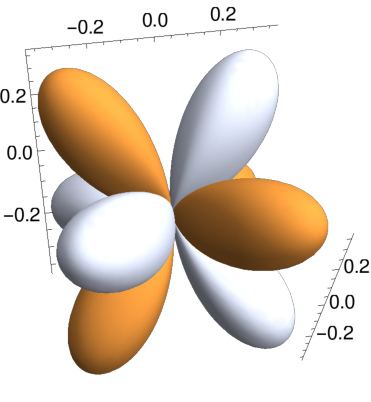
\includegraphics[width=0.4\textwidth]{spindecomptet1}
\caption{Transforms under $A$ (the identity). Clear tetrahedral symmetry.}
\label{figure-spintet1}
\end{figure}

\begin{figure}[H]
\centering
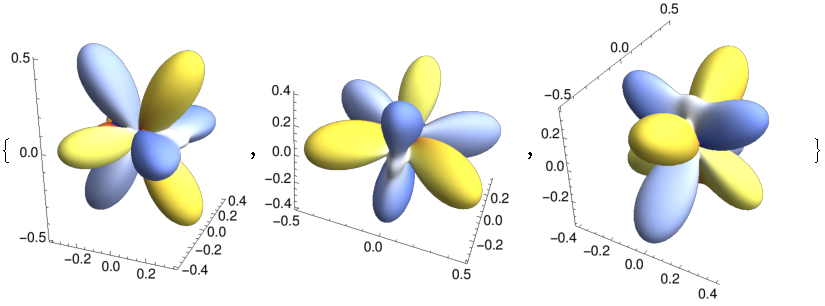
\includegraphics[width=0.7\textwidth]{spindecomptet2}
\caption{Transforms under one copy of  $T$}
\label{figure-spintet2}
\end{figure}
\begin{figure}[H]
\centering
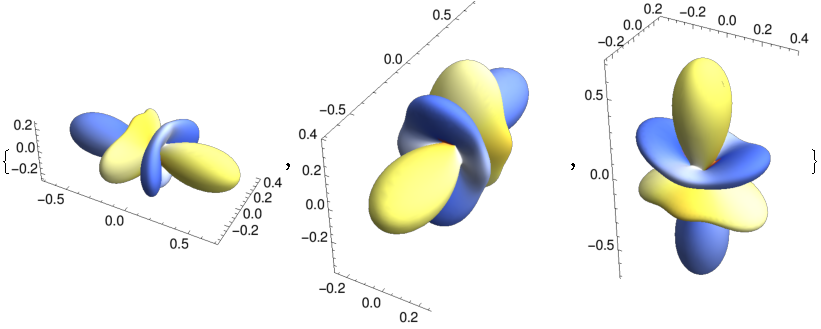
\includegraphics[width=0.7\textwidth]{spindecomptet3}
\caption{Transforms under a different copy of $T$}
\label{figure-spintet3}
\end{figure}
\end{ex}

\begin{ex} Considering icosahedral irreps, $\operatorname{Spin}(6)\cong A\oplus T_1\oplus G\oplus H$. 
  We've found 13 wavefunctions which are a good 
  alternative orthonormal basis for the 13 spherical harmonics.

\begin{figure}[H]
\centering
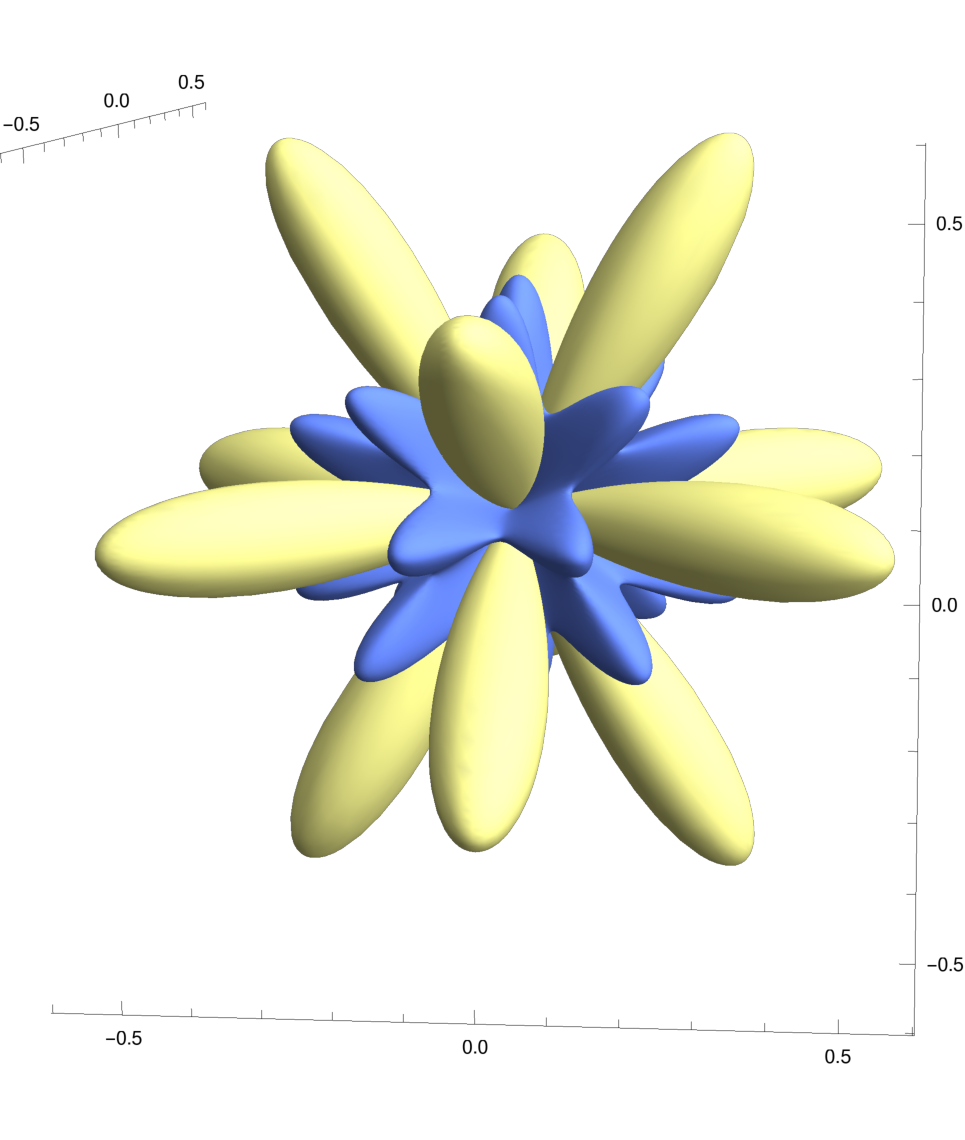
\includegraphics[width=0.4\textwidth]{spindecomp61}
\caption{Transforms under $A$ (the identity). This is the first one out of spin 0 through 5 whose wavefunction has 
such clear icosahedral symmetry.}
\label{figure-spin61}
\end{figure}
  
\begin{figure}[H]
\centering
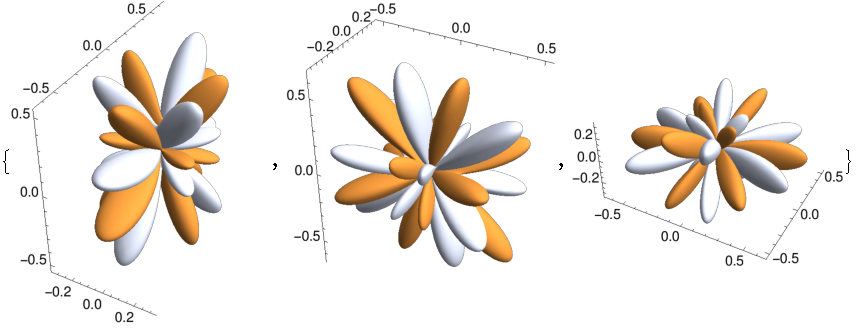
\includegraphics[width=0.7\textwidth]{spindecomp63}
\caption{Transforms under the 3-dimensional irrep $T_1$}
  \label{figure-spin63}
\end{figure}

\begin{figure}[H]
\centering
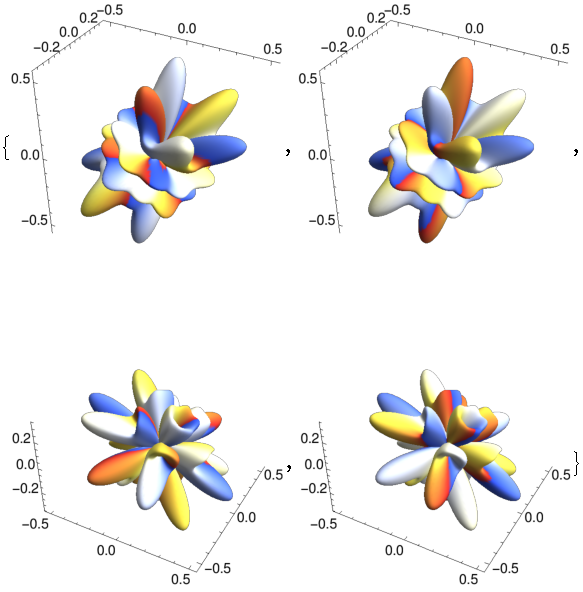
\includegraphics[width=0.5\textwidth]{spindecomp64}
\caption{Transforms under the 4-dimensional irrep $G$}
  \label{figure-spin64}
\end{figure}

\begin{figure}[H]
\centering
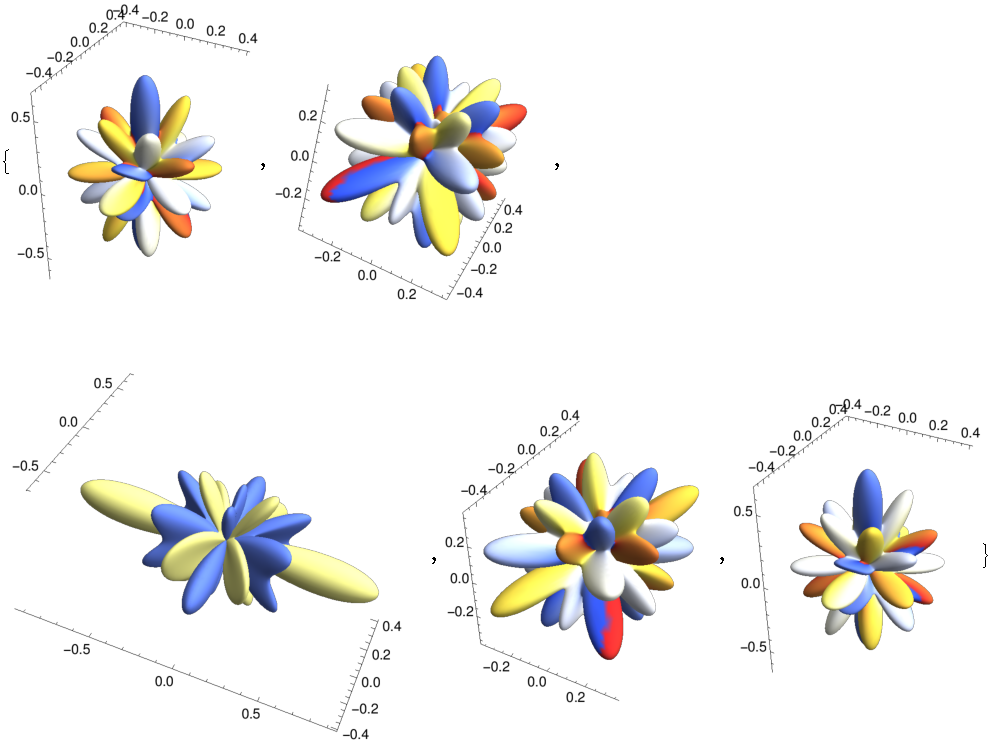
\includegraphics[width=0.7\textwidth]{spindecomp65}
\caption{Transforms under the 5-dimensional irrep $H$}
  \label{figure-spin65}
\end{figure}
\end{ex}


\section{3 Dimensional Point Groups}
\subsection{Basic Definitions}

\begin{defn}
  $O(N)$ is the group of all orthonormal real matrices in $N$ dimensions.
\end{defn}
\begin{defn}
  $SO(N)\leq O(N)$ is the group of all elements of $O(N)$ with determinant 1.
\end{defn}
\begin{defn}
  A \emph{point group} or \emph{finite point group} is a finite subgroup of $O(N)$. Two point groups are equivalent if they are related by conjugation.

  A \emph{proper point group} is a finite subgroup of $O(N)$. 
\end{defn}

\begin{thm}
  The only point groups in $2$ dimensions are $C_n$ (the cyclic group of order 
  $n$) and $D_n$ (the dihedral group on $n$ points).
\end{thm}

\begin{thm}
  The only finite subgroups of the rotation group in 3 dimensions are $C_n$, $D_n$,
  $T$, $O$, and $I$. $T$ is the tetrahedral group, $O$ the octahedral group,
  and $I$ the icosahedral group.
\end{thm}

\begin{proof}
  The $n$-fold axes of a finite subgroup of $SO(3)$ form a regular polyhedron. There are five regular polyhedra, and
  the cube and octahedron correspond to the octahedral group while the icosa- and dodeca- hedron correspond to 
  the icosahedral group. The tetrahedral group remains.
\end{proof}

\begin{note}
  The subgroups of $O(3)$ are much more exhausting! This is because equivalent group structures can have 
  different realizations in 3-space even if they have the same group structure. For example, we could rotate by
  $90^\circ$ about the $\hat{z}$ axis to get $C_4$. We could also rotate by 90 degrees about the $\hat{z}$ axis,
  then reflect across the $\hat{x}\hat{y}$ plane to get a different cyclic group $S_{4}$. As groups they're equivalent (and so
  their character tables are the same),
  but their 3D representations are different.
\end{note}

\begin{defn}
  Sch\"onflies or Schoenflies notation is a convention very useful in writing about
  3-dimensional point groups. It involves the following symbols, each representing 
  a different point group or family of point groups:

  \begin{align*}
 C_n &&  C_{nh} && C_{nv} && S_{2n} &&D_n && D_{nd} && D_{nh} && T && T_d && T_h && O && O_h && I && I_h
  \end{align*}

  $C_n$, $D_n$, $T$, $O$, and $I$ are the proper point groups mentioned earlier.

  $h$ is for ``horizontal'' plane reflection, ``d'' is for ``diagonal'' plane reflection, and ``v'' is for ``vertical'' plane
  reflection. The ``C'' is for ``cyclic'' (even though $C_{nh}$ and $C_{nv}$ aren't cyclic), and the ``S'' is for Spiegel, 
  which is the German word for mirror. The notation is sort of easy to memorize and specific to three dimensions.
\end{defn}

\subsection{Cn, Cnh, Cnv, and S2n}

\begin{defn}
  For this section and the next, define the following four matrices:
  \begin{align*}
    c_n=
  \begin{bmatrix}
    \cos(2\pi/n) & -\sin(2\pi/n) & 0 \\ \sin(2\pi/n) & \cos(2\pi/n) & 0 \\ 0 & 0 & 1
  \end{bmatrix}
  & & \sigma_h=
  \begin{bmatrix}
    1 & 0 & 0 \\ 0 & 1 & 0 \\ 0 & 0 & -1
  \end{bmatrix}
  & & \sigma_v=
  \begin{bmatrix}
    -1 & 0 & 0 \\ 0 & 1 & 0 \\ 0 & 0 & 1
  \end{bmatrix}
  \end{align*}

  $c_n$ is the cyclic generator of order $n$, $\sigma_h$ is a reflection through the horizontal $\hat{x}\hat{y}$ plane, and 
  $\sigma_v$ is a reflection through the vertical $\hat{y}\hat{z}$ plane. These will be our generators.
\end{defn}
\begin{defn}
  If $X$ is a shape in 3D space, the \emph{orbit} of $X$ under a group $G$ is the set of all $gX$ where $g\in G$.
\end{defn}
\begin{defn}
  $C_n$ is the cyclic group of rotations about the $\hat{z}$ axis by an angle $\frac{2\pi}{n}$. It's generated by the single matrix $c_n$. 
  $C_{n}$ has the same group structure as $\mathbb{Z}_n$.
\end{defn}

\begin{defn}
  $C_{nh}$ is the group $C_n$ together with reflections about the horizontal plane. It's generated by the matrices $c_n$ and $\sigma_h$. 
  $C_{nh}$ has the same group structure as $\mathbb{Z}_n\times \mathbb{Z}_2$ (note $\sigma_h$ commutes with $c_n$).
\end{defn}

\begin{defn}
  $C_{nv}$ is the group $C_n$ together with reflections about the horizontal plane. It's generated by the matrices $c_n$ and $\sigma_v$. 
  $C_{nv}$ has the same group structure as the dihedral group $D_n$.
\end{defn}

\begin{defn}
  $S_{2n}$ is cyclic group generated by the matrix $\sigma_hc_n$. These are called ``rotoreflections''.
$S_{2n}$ has the same group structure as $\mathbb{Z}_{2n}$.
\end{defn}

\begin{figure}[H]
\centering
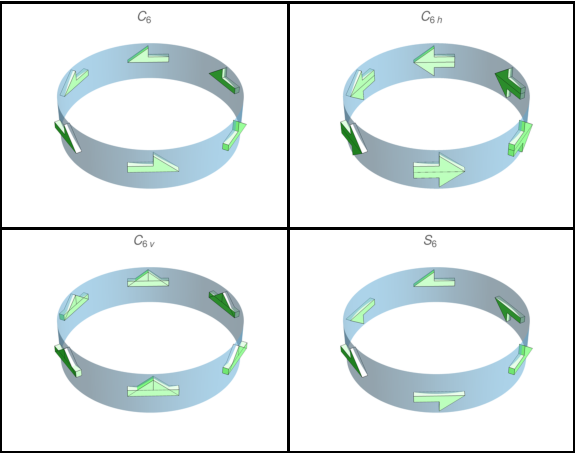
\includegraphics[width=0.9\textwidth]{figureCS}
\caption{Orbits of an arrow under the given C groups}

\label{figure-cs}
\end{figure}

\subsection{Dn, Dnd, and Dnh}
\begin{defn}
  $D_{n}$ is dihedral group. It's generated by the matrix $c_n$, together with rotation by 180 degrees about the $\hat{y}$ direction:
  \begin{equation*}
  \begin{bmatrix}
    -1 & 0 & 0 \\ 0 & 1 & 0 \\ 0 & 0 & -1
  \end{bmatrix}
\end{equation*}

  Note that this matrix is equal to $\sigma_h\sigma_v$
\end{defn}

\begin{defn}
  $D_{nd}$ is the point group generated by $c_{2n}\sigma_h$ and $\sigma_v$. It contains $C_n$, $C_{nh}$, $C_{nv}$, $S_{n}$, and $D_n$.
  $D_{nd}$ actually has the same group structure as the dihedral group on $2n$ points, $D_{2nd}$.
\end{defn}

\begin{defn}
  $D_{nh}$ is the point group generated by $c_n$, $\sigma_v$, and $\sigma_h$. It's a subgroup of $D_{2n}$.
  As a group, $D_{nh}$ is isomorphic to $D_n \times \mathbb{Z}_2$. 
\end{defn}


\begin{figure}[H]
\centering
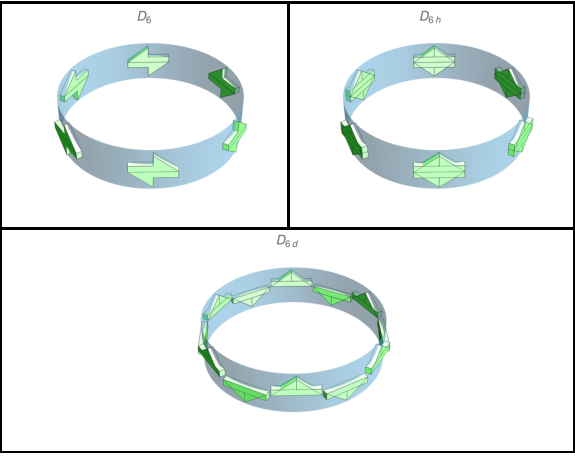
\includegraphics[width=0.9\textwidth]{figureD}
\caption{Orbits of an arrow under the given D groups}

\label{figure-d}
\end{figure}

\subsection{T, Td, and Th}

\begin{defn}
  For this section, we care about different rotations and translations. Consider the tetrahedron with
  vertices at $(1,1,1)$, $(-1,-1,1)$, $(-1,1,-1)$, and $(1,-1,-1)$. The symmetries of this set of points are:
  rotation by $180^\circ$ about the $\hat{z}$ axis; rotation by $120^\circ$ about the $(1,1,1)$ axis;
  reflection through the plane spanned by $(1,1,0)$ and $(0,0,1)$; and finally inversion. These four matrices are, respectively:
  \begin{align*}
    r_2=
  \begin{bmatrix}
    -1& 0 & 0 \\ 0 & -1 & 0 \\ 0 & 0 & 1
  \end{bmatrix}
  & & r_3=
  \begin{bmatrix}
    0 & 0 & 1 \\ 1 & 0 & 0 \\ 0 & 1 & 0
  \end{bmatrix}
  & & \sigma=
  \begin{bmatrix}
    0 & 1 & 0 \\ 1 & 0 & 0 \\ 0 & 0 & 1
  \end{bmatrix}
  & & \iota=
  \begin{bmatrix}
    -1& 0 & 0 \\ 0 & -1 & 0 \\ 0 & 0 & -1
  \end{bmatrix}
  \end{align*}
\end{defn}

\begin{defn}
  $T$ is the point group generated by $r_2$ and $r_3$. As a group it is isomorphic to $A_4$. It has twelve elements.
\end{defn}

\begin{defn}
  $T_d$ is the point group generated by $r_2$, $r_3$, and $\sigma$. As a group it is isomorphic to $S_4$. It has 24 elements.
\end{defn}

\begin{defn}
  $T_h$ is the point group generated by $r_2$, $r_3$, and $\iota$. As a group it is isomorphic to $A_4\times \mathbb{Z}_2$ (Note that $\iota$ commutes with $r_2$ and $r_3$). It has 24 elements.
\end{defn}

\begin{figure}[H]
\centering
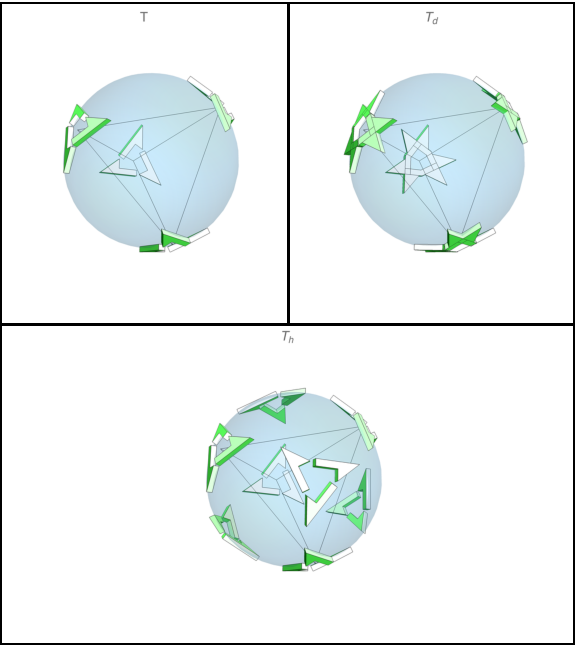
\includegraphics[width=0.9\textwidth]{figureT}
\caption{Orbits of an arrow under the given T groups, together with a plot of the underlying tetrahedron.}

\label{figure-t}
\end{figure}

\subsection{O and Oh}

\begin{defn}
  The proper octahedral point group $O$ can be generated by rotation by $\pi/2$ about any two principal axes. For example, 

  \begin{align*}
    \begin{bmatrix}
       1 & 0 & 0 \\ 0 & 0 & -1 \\ 0 & 1 & 0
    \end{bmatrix} & &  
    \begin{bmatrix}
      0 & 0 & 1 \\ 0 & 1 & 0 \\ -1 & 0 & 0
    \end{bmatrix} 
  \end{align*}
  As a group it is isomorphic to $S_4$.
\end{defn}

\begin{defn}
  The improper octahedral point group $O_h$ can be generated by the generators of $O$ as well as inversion symmetry $\iota$. 
  As a group it is isomorphic to $S_4\times \mathbb{Z}_2$.
\end{defn}

\begin{figure}[H]
\centering
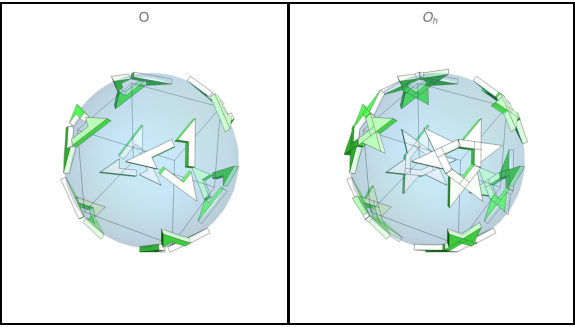
\includegraphics[width=0.9\textwidth]{figureO}
\caption{Orbits of an arrow under the given O groups. A cube is also plotted for reference. Note how
the diagram for O differs from that for $T_h$.}

\label{figure-o}
\end{figure}
\subsection{I and Ih}

\begin{defn}
  The proper Icosahedral point group $I$ can be generated by rotation by $\pi$ in the $\hat{x}\hat{y}$ plane, as well as a 
  rotation by $72^\circ$. If we denote $f=(1+\sqrt{5})/2$, then we have the following two generators:
  \begin{align*}
    \begin{bmatrix}
       -1 & 0 & 0 \\ 0 & -1 & 0 \\ 0 & 0 & 1
    \end{bmatrix} & &  
    \frac{1}{2}
    \begin{bmatrix}
      1 & -f & 1/f \\ f & 1/f & -1 \\ 1/f & 1 & f
    \end{bmatrix} 
  \end{align*}
  As a group it is isomorphic to $A_5$.
\end{defn}

\begin{defn}
  The improper icosahedral point group $O_h$ is generated by the generators of $I$ as well as inversion symmetry $\iota$. 
  As a group it is isomorphic to $A_5\times \mathbb{Z}_2$.
\end{defn}


\begin{figure}[H]
\centering
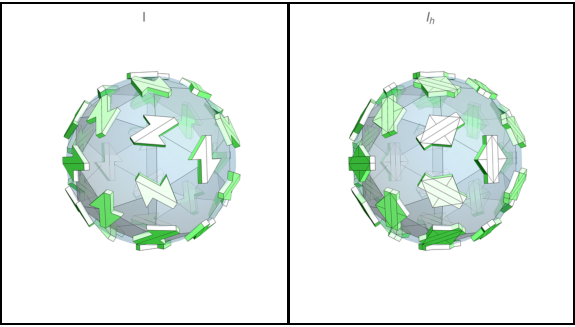
\includegraphics[width=0.9\textwidth]{figureI}
\caption{Orbits of an arrow under the given I groups. A partially opaque icosidodecahedron is 
also plotted, in an attempt to make the diagram more clear.}

\label{figure-i}
\end{figure}






\section{An Elementary look at Carbon C60}

\subsection{A Sphere with a Weak Icosahedral Potential}

\subsection{A Tight Binding Model}

\subsection{A Spring-and-Ball Model}

\section{Wigner-Eckart theorem}


\section{Lattices}

\subsection{Basic Theory}

\subsection{Application to condensed matter systems}

test

\end{document}
